\section{Sumador completo \label{sec:s2}}

\begin{center}
	\begin{minipage}{12cm}
		\begin{tcolorbox}[title=Actividad 2]
			Codificar el sumador completo (con acarreo de entrada y acarreo de salida) indicado en la lámina 11, en los dos lenguajes y compilar. Alguno presenta algún error durante la compilación. ¿Cómo se soluciona el problema?
		\end{tcolorbox}	
	\end{minipage}
\end{center}

Se presenta un error en VHDL, como se observa en la \autoref{fig:full_adder_vhdl_error}, esto surge debido a que se necesita que los operandos sean del mismo tamaño que la variable en donde se almacenará el resultado. Para solucionarlo, unicamente se necesita concatenar un bit, en bajo, en la posición más significativa de ambos operandos. Este error no sucede con Verilog, ya que el propio lenguaje concatena el bit faltante automáticamente.

\begin{figure}[ht]
	\centering
	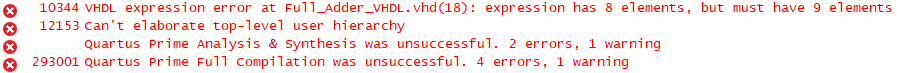
\includegraphics[scale=0.7]{Full_Adder_VHDL_Error.png}
	\caption{Error obtenido al utilizar el código de la lámina 11 sin modificar. \label{fig:full_adder_vhdl_error}}
\end{figure}

La visualización RTL del sumador completo en VHDL se muestra en la \autoref{fig:full_adder_vhdl_rtl} y en Verilog en la \autoref{fig:full_adder_verilog_rtl}. Las simulaciones para el código en VHDL se visualizan en la \autoref{fig:full_adder_vhdl_WaveBi} en base binaria y en la \autoref{fig:full_adder_vhdl_WaveDe} en base decimal. En cambio, las simulaciones para el código en Verilog se visualizan en la \autoref{fig:full_adder_verilog_WaveBi} en base binaria y en la \autoref{fig:full_adder_verilog_WaveDe} en base decimal. Los valores empleados son los mismos que los de la Actividad 1.

\begin{figure}[ht]
	\centering
	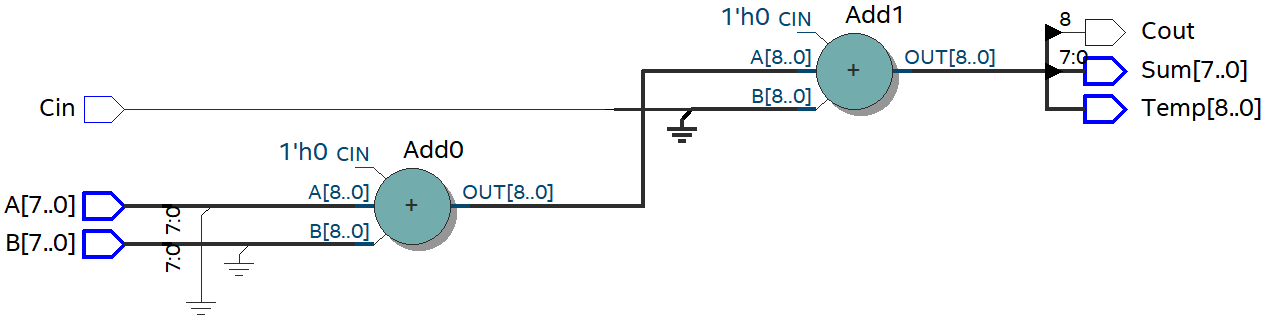
\includegraphics[scale=0.5]{Full_Adder_VHDL_RTL.png}
	\caption{Diagrama RTL del sumador completo en VHDL. \label{fig:full_adder_vhdl_rtl}}
\end{figure}

\begin{figure}[ht]
	\centering
	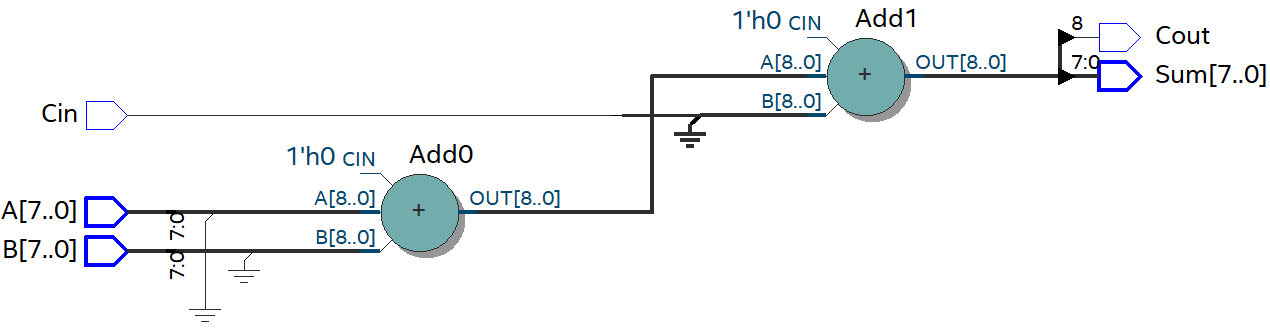
\includegraphics[scale=0.5]{Full_Adder_Verilog_RTL.png}
	\caption{Diagrama RTL del sumador completo en Verilog. \label{fig:full_adder_verilog_rtl}}
\end{figure}

\begin{figure}[ht]
	\centering
	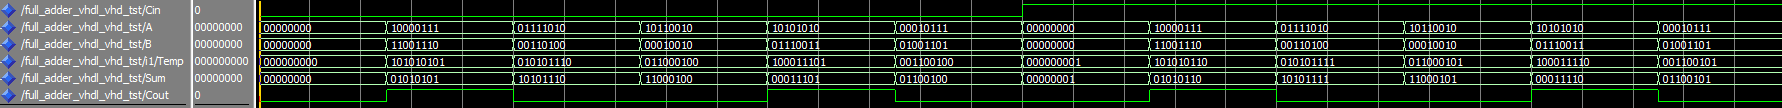
\includegraphics[scale=0.35]{Full_Adder_VHDL_WaveBi.png}
	\caption{Simulación del sumador completo en VHDL con el visor de formas de onda de ModelSim (Base binaria). \label{fig:full_adder_vhdl_WaveBi}}
\end{figure}

\begin{figure}[ht]
	\centering
	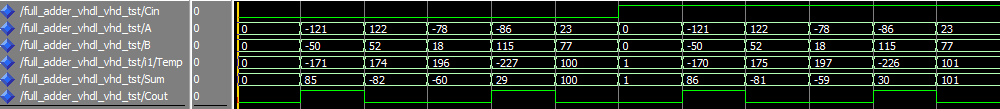
\includegraphics[scale=0.6]{Full_Adder_VHDL_WaveDe.png}
	\caption{Simulación del sumador completo en VHDL con el visor de formas de onda de ModelSim (Base decimal). \label{fig:full_adder_vhdl_WaveDe}}
\end{figure}

\begin{figure}[ht]
	\centering
	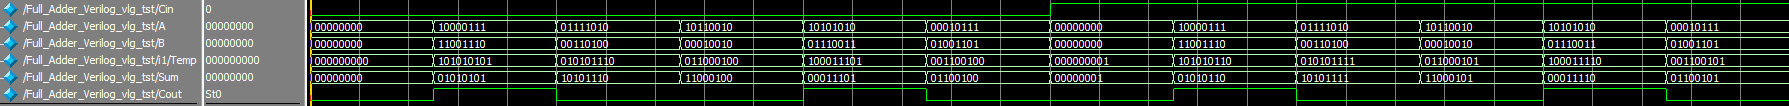
\includegraphics[scale=0.35]{Full_Adder_Verilog_WaveBi.png}
	\caption{Simulación del sumador completo en Verilog con el visor de formas de onda de ModelSim (Base binaria). \label{fig:full_adder_verilog_WaveBi}}
\end{figure}

\begin{figure}[ht]
	\centering
	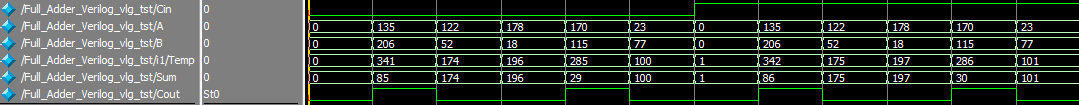
\includegraphics[scale=0.6]{Full_Adder_Verilog_WaveDe.png}
	\caption{Simulación del sumador completo en Verilog con el visor de formas de onda de ModelSim (Base decimal). \label{fig:full_adder_verilog_WaveDe}}
\end{figure}





